\documentclass[a4paper, twocolumn]{article}
\setlength{\columnsep}{40pt}
\usepackage{graphicx} 
\usepackage[a4paper,margin=0.5in]{geometry}
\usepackage{amsmath}

\begin{document}

\title{Data Visualization on the Titanic Dataset}
\author{Jawadul Chowdhury}
\date{\today}
\maketitle

\section{Abstract}
To be worked on.

\section{Introduction}
The Titanic was a British passenger ship that sank in the Atlantic Ocean on April 15, 1912. The ship had struck an 
iceberg on its maiden voyage from Southampton, England to New York City. \\

We use exploratory data analysis on the titanic dataset, using different visualizatoin tehcniques as well as
determining which features are should be included in a machine learning model.

\section{Dataset Description}
When examining the dataset, there are a total of 16 features. Such 
variables are listed as follows:

\begin{itemize}
    \item \texttt{PassengerId}: The ID of the passenger. This is a discrete numerical data type as the difference
     between units is constant.
    \item \texttt{Survived}: Whether the passenger survived or not.This is a nominal binary categorical data type 
    as there is no order information. 0 means passenger didn't survive and and 1 means passenger did survive.
    \item \texttt{Pclass}: This is the passenger class. It is a ordinal categorical data type, as 1 means 1st ticket 
    class and so on for 2 and 3, to identify passenger class.
    \item \texttt{Name}: The name of the passenger. This is a  nominal categorical data type, as the names of the 
    passenger have no order information.
    \item \texttt{Sex}: This is the sex of the passenger. This is a nominal categorical data type,as genders can't be 
    ordered and is rather binary.
    \item \texttt{Age}: Age of the Passenger. This is a continuous numerical data type, as the difference between 
    units is constant and can be counted.
    \item \texttt{SibSp}: Number of Siblings / Spouses of the passenger. It is a discrete numerical data type as it 
    can be counted and has a constant difference between units.
    \item \texttt{Parch}: Number of Parents / Children abroad the Titanic. It is a discrete numerical data type, as 
    it can be counted and can only take certain values.
    \item \texttt{Ticket}: This is the ticket number. This is a  nominal categorical data type as there is no ordering 
    information.
    \item \texttt{Fare}: This is the passenger fare. This is a ratio numerical data type as there is a true zero, 
    where zero means that the passenger has not paid any fare.
    \item \texttt{Cabin}: This is the cabin number of the passenger. It is a nominal categorical data type as there 
    is no order information bur rather a quantitvate classifcation.
    \item \texttt{Embarked}: This is the port where the passenger embarked. C is Cherbourg, Q is Queenstown and S 
    is Southampton. This is a categorical nominal data type as there is no order information and has quantitative 
    classification.
    \item \texttt{Age\_fill\_mean}: This is a copy of the Age column but the blanks have been filled in with the mean.
    This is a ratio numerical data type, because there are  fractional values and has a true zero point.
    \item \texttt{Age\_fill\_median}: This is a copy of the Age column but the blanks have been filled in with the
    median. This is a discrete numerical data type because the age is defined to be continuous numerical.
    \item \texttt{Age\_fill\_mode}: This is a copy of the Age column but the blanks have been filled in with the mode.
    This is a discrete numerical data type, because the age is defined to be continuous numerical.
    \item \texttt{Age\_fill\_knn}: This is a copy of the Age column but the blanks have been filled in with the mean.
    This is a ratio numerical data type, because there are fractional values and has a true zero point.
\end{itemize}

\section{Data Visualization on Survived}
Now, we move on to visualizting some of the variables we have in the Titanic dataset against the \texttt{Survived}
variable. We also look for any predictive relationships using the plots.

\subsection{Fare vs Survived}
In order to determine a appropriate plot type, we need to identify the type of data. We know that the 
\texttt{Survived} variable is binary and categorical, and we know that \texttt{Fare} is a ratio numerical data type.
For this application, it would be best to use a box plot since we're dealing with categorical / numerical data, as 
shown in Figure 1.



\begin{figure}[h!] 
    \centering
    \noindent
    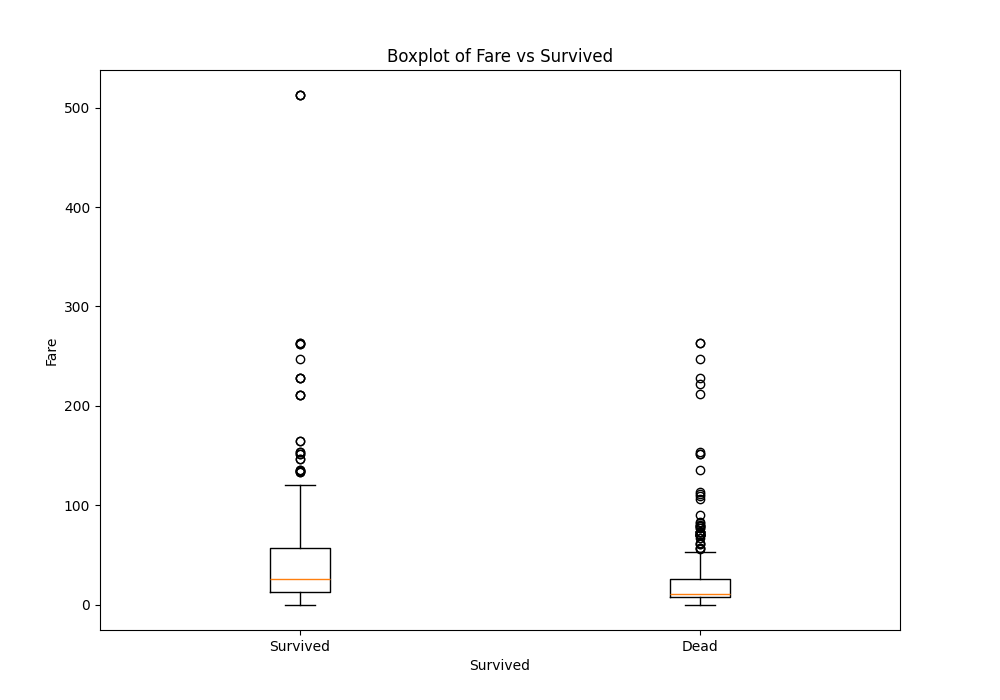
\includegraphics[width=\columnwidth]{C:/GitHub/DataScience/wk_03/plots/BoxPlotFareSurvived.png}  
    \caption{Box Plot of Fare vs Survived} 
\end{figure}

\subsection{Sex vs Survived}
Next up, we now plot the \texttt{Sex} variable against \texttt{Survived} variable. We know that the \texttt{Sex}
variable is a categorical variable, which uses male and female. We also have the survived variable which is also
categorical as discussed previously. For this application, we can use a Heat Map since we're dealing with categorical
/ categorical data as shown in Figure 2.
\begin{figure}[h!] 
    \centering
    \noindent
    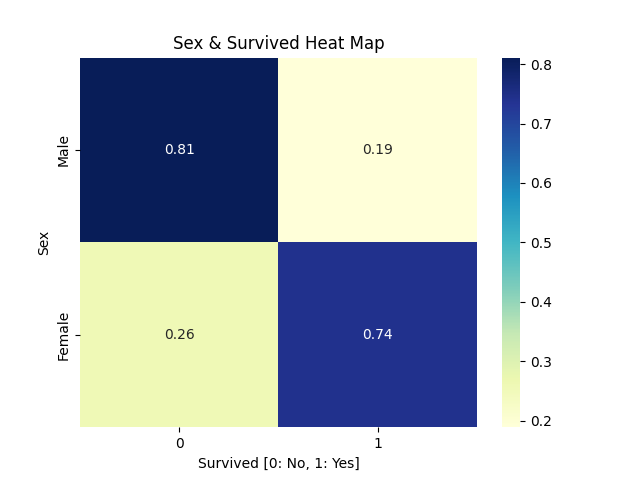
\includegraphics[width=\columnwidth]{C:/GitHub/DataScience/wk_03/plots/HeatMapSexSurvived.png}  
    \caption{Heat Map of Sex vs Survived} 
\end{figure}

\subsection{Sibling / Spouse vs Survived}
Next up, we now plot the \texttt{SibSp} variable against the \texttt{Survived} variable. We know that the
\texttt{SibSp} variable is a discrete numerical data type, as it can be counted. As a result, since we're plotting
a numerical data type against a categorical data type, we can use a bot plot to best represent this numerical 
/ categorical data as shown in Figure 3.
\begin{figure}[h!] 
    \centering
    \noindent
    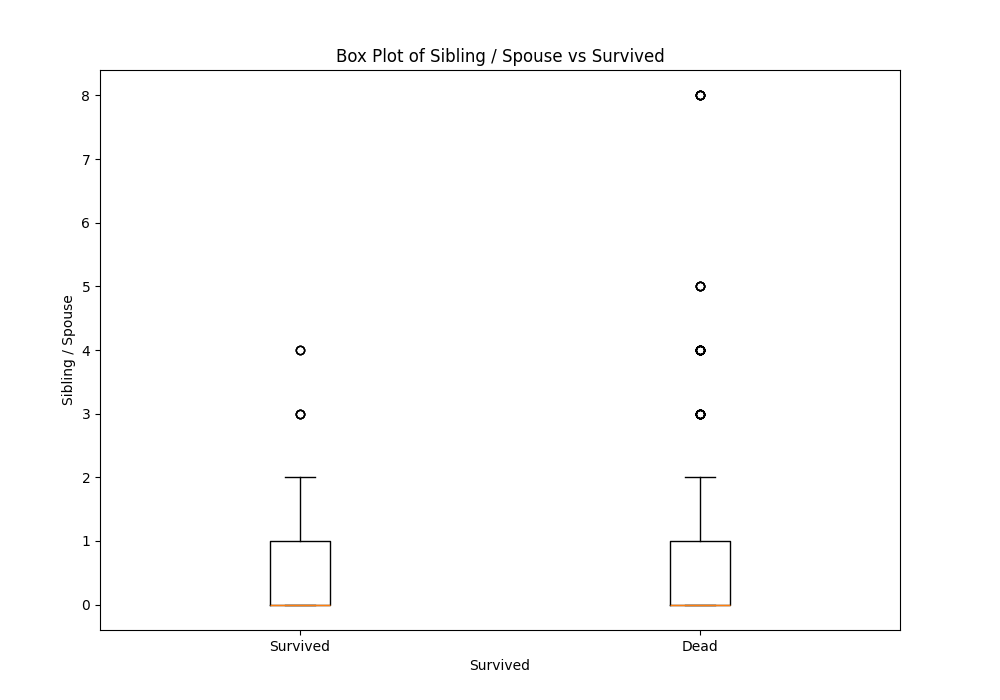
\includegraphics[width=\columnwidth]{C:/GitHub/DataScience/wk_03/plots/BoxPlotSibSpSurvived.png}  
    \caption{Heat Map of Sibling / Spouse vs Survived} 
\end{figure}

\subsection{Parent / Children vs Survived}
Moreover, we now plot the \texttt{Parch} variable against the \texttt{Survived} variable. We know that the 
\texttt{Parch} variable is a discrete numerical data type, as it can be counted. As a result, since we're plotting
a numerical data type against a categorical data type, we can use a bot plot to best represent this as shown in 
Figure 4.
\begin{figure}[h!] 
    \centering
    \noindent
    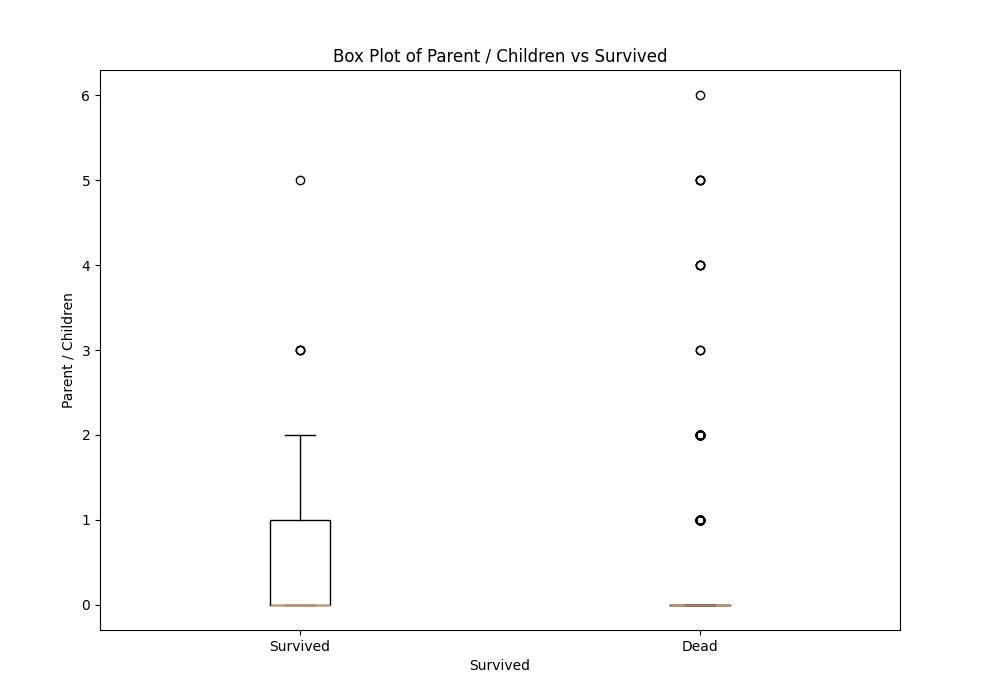
\includegraphics[width=\columnwidth]{C:/GitHub/DataScience/wk_03/plots/BoxPlotParchSurvived.png}  
    \caption{Heat Map of Parent / Children vs Survived} 
\end{figure}

\subsection{Embarked vs Survived}
Moving on, we now plot the \texttt{Embarked} variable against the \texttt{Survived} variable. We know that the 
\texttt{Embarked} variable is a categorical data type, and since we're plotting the a categorical data type against
a categorical data type, we can then use a heat map to best represent this as shown in Figure 5.
\begin{figure}[h!] 
    \centering
    \noindent
    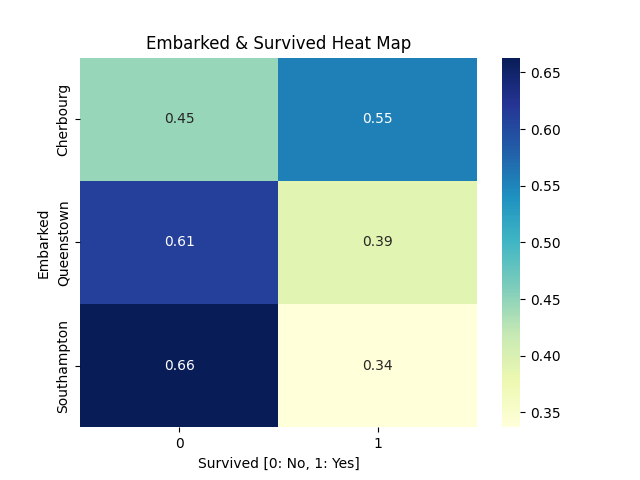
\includegraphics[width=\columnwidth]{C:/GitHub/DataScience/wk_03/plots/HeatMapEmbarkedSurvived.png}  
    \caption{Heat Map of Parent / Children vs Survived} 
\end{figure}

\subsection{Passenger Class vs Survived}
Next, we now plot the \texttt{Pclass} variable against the \texttt{Survived} variable. We know that the 
\texttt{Pclass} variable is a categorical data type, and since we're plotting the a categorical data type against
a categorical data type, we can then use a heat map to best represent this as shown in Figure 6.
\begin{figure}[h!] 
    \centering
    \noindent
    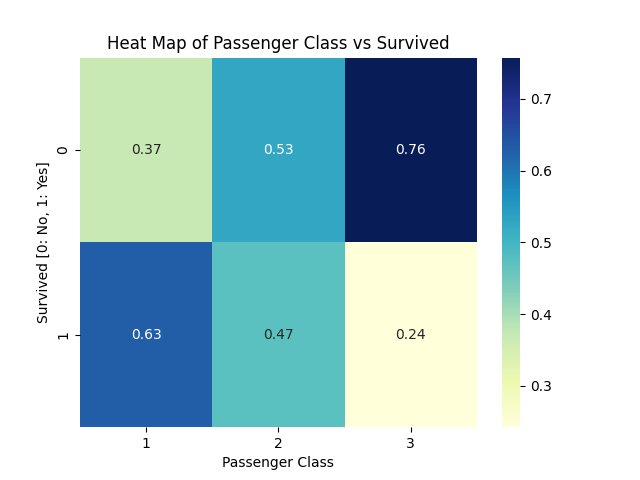
\includegraphics[width=\columnwidth]{C:/GitHub/DataScience/wk_03/plots/PClassVsSurvivedHeatMap.png}  
    \caption{Heat Map of Parent / Children vs Survived} 
\end{figure}

\subsection{Age Fill Mean vs Survived}
Now, we plot the \texttt{Age\_fill\_mean} variable against the \texttt{Survived} variable. We know that the 
\texttt{Age\_fill\_mean} is a ratio numerical data type and \texttt{Survived} is a categorical data type.
To create a plot where we plot a categorical data type against a numerical data type, we can use a violin plot, as
shown in Figure 7.
\begin{figure}[h!] 
    \centering
    \noindent
    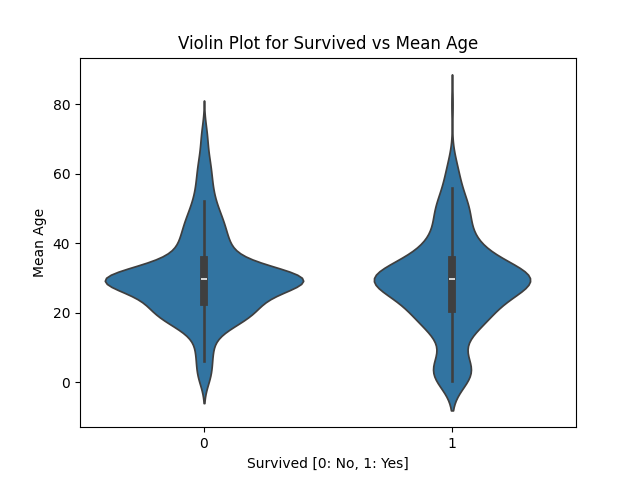
\includegraphics[width=\columnwidth]{C:/GitHub/DataScience/wk_03/plots/ViolionPlotSurvivedMean.png}  
    \caption{Violin Plot of Age (Mean) vs Survived} 
\end{figure}

\subsection{Age Fill KNN vs Survived}
Now, we plot the \texttt{Age\_fill\_KNN} variable against the \texttt{Survived} variable. We know that the 
\texttt{Age\_fill\_KNN} is a ratio numerical data type and \texttt{Survived} is a categorical data type.
To create a plot where we plot a categorical data type against a numerical data type, we can use a violin plot, as
shown in Figure 8.
\begin{figure}[h!] 
    \centering
    \noindent
    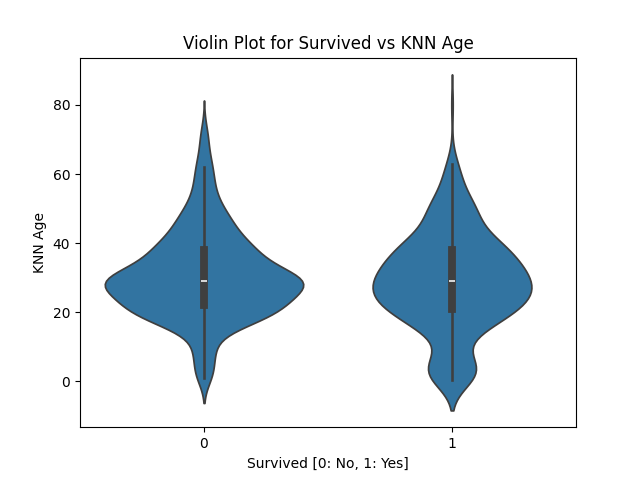
\includegraphics[width=\columnwidth]{C:/GitHub/DataScience/wk_03/plots/ViolinPlotKNNSurvived.png}  
    \caption{Violin Plot of Age (KNN) vs Survived} 
\end{figure}

\subsection{Age Fill Median vs Survived}
Next, we plot the \texttt{Age\_fill\_Median} variable against the \texttt{Survived} variable. We know that the 
\texttt{Age\_fill\_Median} is a discrete numerical data type and \texttt{Survived} is a categorical data type.
To create a plot where we plot a categorical data type against a numerical data type, we can use a violin plot, as
shown in Figure 9.
\begin{figure}[h!] 
    \centering
    \noindent
    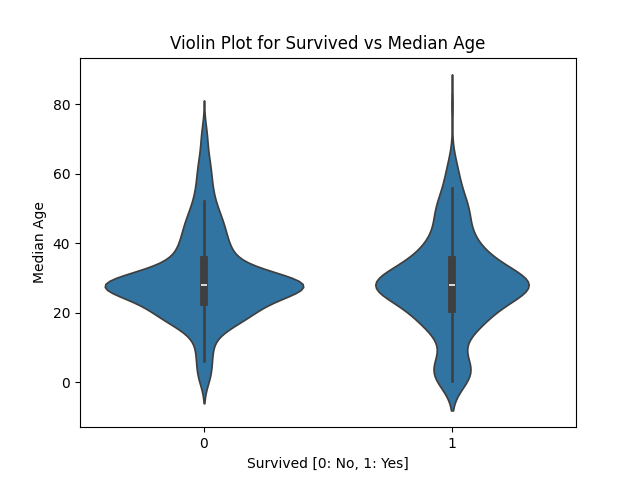
\includegraphics[width=\columnwidth]{C:/GitHub/DataScience/wk_03/plots/ViolionPlotSurvivedMedian.png}  
    \caption{Violin Plot of Age (Median) vs Survived} 
\end{figure}

\subsection{Age Fill Mode vs Survived}
Lastly, we plot the \texttt{Age\_fill\_Mode} variable against the \texttt{Survived} variable. We know that the 
\texttt{Age\_fill\_Mode} is a discrete numerical data type and \texttt{Survived} is a categorical data type.
To create a plot where we plot a categorical data type against a numerical data type, we can use a violin plot, as
shown in Figure 10.
\begin{figure}[h!] 
    \centering
    \noindent
    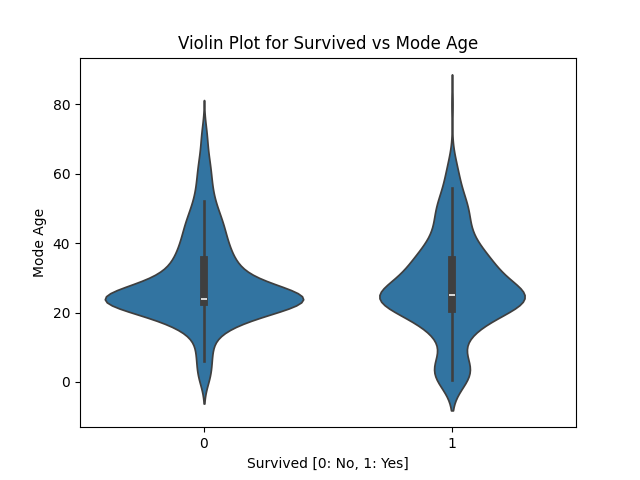
\includegraphics[width=\columnwidth]{C:/GitHub/DataScience/wk_03/plots/ViolionPlotSurvivedMode.png}  
    \caption{Violin Plot of Age (Mode) vs Survived} 
\end{figure}


\section{Relationships}
Now that we have produced the graphs, we need to understand the predictive relationships that can be analyzed 
from them. In order to do this, we look at each visualization that has been produced.

\subsection{}

\section{Sources}



\end{document}
